\documentclass[10pt]{article}

\usepackage{rlc}
% If accepted, instead use the following line for the camera-ready submission:
%\usepackage[accepted]{rlc}
% To de-anonymize and remove mentions to RLC (for example, for posting to preprint servers), instead use the following:
% \usepackage[preprint]{rlc}

\usepackage{array}
\usepackage{amsmath}
\usepackage{amsthm}
\usepackage{amsbsy}
\usepackage{amssymb}
\newtheorem{definition}{Definition}
\usepackage{graphicx}
\usepackage{mathtools}
\usepackage{nicefrac}
\usepackage{bm}
\usepackage{enumitem}
\usepackage{mpemath}
\usepackage{tcolorbox}
\usepackage[capitalize,noabbrev]{cleveref}
\usepackage{theoremref}
\usepackage{thmtools}
\usepackage{thm-restate}
\usepackage{algorithm}
\usepackage{algpseudocode}
\usepackage{tikz}

\bibliographystyle{abbrvnat}
\usepackage[framemethod=default]{mdframed}

\renewcommand{\cite}{\citep}

%\mathtoolsset{showonlyrefs}     % Only number equations that are referenced (optional)

\renewcommand{\algorithmicrequire}{\textbf{Input:}}
\renewcommand{\algorithmicensure}{\textbf{Output:}}
\newtheorem{theorem}{Theorem}
\newtheorem{lemma}{Lemma} 
\newtheorem{proposition}{Proposition}
\newtheorem{assumption}{Assumption}

\newcommand{\mm}[1]{\textcolor{blue}{[#1]}}
\newcommand{\gersi}[1]{\textcolor{red}{[#1]}}
\newcommand{\s}[1]{\mathcal{#1}}

\DeclareMathOperator{\ext}{ext}

\setlength{\parskip}{3mm plus 1mm minus 1mm}
\setlength{\parindent}{0pt}

\title{ROIL: Robust Inverse Reinforcement Learning Without Trajectories}
\author{Gersi Doko \\
        Gersi.Doko@unh.edu \\
        \and 
        Marek Petrik \\
        mpetrik@cs.unh.edu \\
        Daniel Brown }

% Relevant emails
% Daniel Brown = daniel.s.brown@utah.edu
% Guang = u1326446@utah.edu

\begin{document}

\maketitle

\begin{abstract}
We study inverse reinforcement learning where the agent attempts to learn an expert's policy from a dataset of collected state, action tuples. We derive a new robust model-based offline Imitation Learning method (ROIL) that mitigates covariate shift by avoiding estimating the expert's occupancy frequency. Frequently in offline settings, there is insufficient data to reliably estimate the occupancy frequency and this leads to models that do not generalize well. Expert demonstrators may also be biased, or worse, adversarial. We propose ROIL, a method that is guaranteed to recover the occupancy frequency and is efficiently solvable as an LP. We demonstrate ROIL's ability to perform well in a large grid world environment even when the state visitation frequency comes from a completely random policy.
\end{abstract}

\section{Introduction}

\emph{Imitation learning} seeks to compute a good policy in a Markov decision process~(MDP) without knowing the reward function. Instead, one only has access to a set of demonstrations performed by a domain expert~\cite{chang2021mitigating, Panaganti2023, Spencer2021, Rashidinejad2022}. Imitation learning promises techniques that can learn to act well in environments where describing an appropriate reward function may be challenging or impractical. Robotics, medicine, and autonomous driving and examples of problem domains that can benefit greatly from more reliable imitation learning algorithms. 

Inverse Reinforcement Learning~(IRL) is a common approach to imitation learning~\cite{abbeel2004, Javed2021, Brown2020, Brown2018b, Brown2018a}. IRL leverages the environment's dynamics modeled as an MDP to efficiently mimic the observed policy of the expert~\cite{Arora2020}. The environment's dynamics may be known a priori~\cite{Syed2008, lacotte2019} or estimated from data~\cite{chang2021mitigating, Ho2016}. An important strength of IRL algorithms is that they can learn to mimic experts quite well even with remarkably little data. However, most IRL algorithms can be very sensitive to the state distribution in the training data. If the distribution of states present in the dataset does not follow the occupancy frequency---a phenomenon known as \emph{covariate shift}---the IRL algorithm may compute a policy that is much worse than the expert's policy. 

In this paper, we propose ROIL, a new approach to IRL that is particularly resistant to any covariate shift. In particular, ROIL allows for data with a state distribution that does not follow the expert's occupancy frequency. Most existing algorithms are sensitive to covariate shift because, in some form, they reduce to matching the expert's state occupancy frequency. In comparison, ROIL attempts to recover the set of expert's plausible policies from the training data and compute a policy that minimizes the regret with respect to this set of experts.

The regret minimization problem at the heart of ROIL is equivalent to finding the \emph{Chebyshev center} of the set of policies consistent with the observed training data. Computing the Chebyshev center of a set corresponds to finding the center of the smallest circumcircle of a set and is NP-hard in general for polyhedral sets described by linear constraints. However, with an appropriate choice of modeling assumption, we show that ROIL can be formulated as a convex optimization problem and solved using mature solvers.

There are several reasons for why the expert demonstration data may not be sampled according to the true occupancy frequency. First, the expert's initial state distribution may differ from the initial state distribution when the learned policy is deployed. Second, the expert may focus on providing demonstrations that focus on the most challenging parts of the state space. The demonstrations may not even form a trajectory but instead consist of disconnected state-action pairs. The state distribution of the demonstrations may differ simply due to sampling and model errors and inconsistencies. These demonstrations can be noisy and may not be representative of the expert's true policy. As a result, one must be careful in solving the primal IL formulation to make it tractable.

To better illustrate the importance of covariate shift, consider the following extreme example. In an MDP with a small state space and the ability to jump between states, the expert provides a single demonstration for each state showing the optimal actions. Behavior cloning algorithms, which reduce imitation learning to a classification problem, will recover the optimal policy given that the classification bias is general enough. Yet, most common IRL algorithms based on the same scheme as LPAL~\cite{Syed2008} or GAIL~\cite{Ho2016} can fail to recover a good policy, as we show below. ROIL, on the other hand, recovers the optimal policy even in this extreme setting while preserving most of the benefits of the low sample complexity of IRL.

ROIL builds on the same ideas as most modern IRL algorithms and can be readily integrated with the improvements developed in recent years~\cite{Arora2020}. As with most IRL algorithms, ROIL seeks to minimize the regret to the expert's policy for the worst-case plausible reward functions. However, ROIL departs significantly from existing IRL algorithms in that it does not directly use the estimate of experts's occupancy frequencies. In contrast, ROIL uses the training data to construct a robust set of plausible expert policies and minimizes the regret of the computed policy in the context of this set. As a result, ROIL cannot be seen as matching the expert's feature frequencies, which is a popular view of existing IRL techniques~\cite{abbeel2004,Syed2008,Ho2016}.
%marek: check if this is still true \gersi{We just said this in paragraph 3}. 

The remainder of the paper is organized as follows. \Cref{sec:preliminaries} describes the background in MDPs and IRL necessary to introduce ROIL. Then, in \cref{sec:optimization-formulation}, we describe our general framework, analyze its basic properties, and propose an optimization algorithm. \Cref{sec:covar-shift-bounds} generalizes the approach to allow for custom bounds on the errors in covariate shift. This extension also helps to make a connection with existing IRL methods. Finally, in \cref{sec:experimental-results}, we analyze ROIL numerically and compare it with relevant algorithms. 

\section{Preliminaries}\label{sec:preliminaries}

Before describing the underlying MDP framework~\cite{Puterman1994} and formally define the IRL problem~\cite{abbeel2004,Syed2008,Ho2016}, we define the basic notation we use in the paper. We use calligraphic letters to denote sets and a tilde to denote random variables. We also adopt the standard convention that $\mathcal{A}^{\mathcal{B}}$ represents the set of all functions from a set $\mathcal{B}$ to a set $\mathcal{A}$. Finally, the sets $\Real$ and $\Real_+$ represent real and non-negative numbers respectively. 


%This introduction is not meant to be exhaustive, but rather to provide the reader with the necessary background to understand the rest of the paper.
%Much of the MDP material comes from~\cite{Puterman1994}.
%For a more in-depth treatment of the IRL setting we refer the reader to~\cite{abbeel2004}.

% \paragraph{Markov Decision Processes}

As is usual in IRL literature, we assume that the domain can be modeled as a \emph{Markov Decision Process} with a finite number of states $\mathcal{S} = \left\{ 1, \dots , S \right\}$ and a finite number of actions $\mathcal{A} = \left\{ 1, \dots , A \right\}$. The transition probability function $p\colon \mathcal{S} \times \mathcal{A} \to \Delta^{\mathcal{S}}$, where $\Delta^{\mathcal{S}} = \left\{ x\in \Real_{+}^S \mid \sum_{s\in \mathcal{S}} x_s =1 \right\}$ is the probability simplex over the elements of the set $\mathcal{S}$. The reward function $r\opt \colon \mathcal{S} \times \mathcal{A} \to \Real$ represents the reward obtained in each transition. The initial distribution over states is denoted by $p_0\in \Delta^S$. 

A solution to an MDP is a \emph{policy}. In this work, we restrict our attention to \emph{stationary randomized} and \emph{deterministic} policies. The set of deterministic policies is $\Pi_D= \mathcal{A}^{\mathcal{S}}$ and the set of randomized policies is $\Pi_R = {\left(\Delta^{\mathcal{A}}\right)}^{\mathcal{S}}$. Note that randomized policies are a special case of deterministic policies. 

We assume the $\gamma$-discounted infinite horizon objective with $\gamma \in [0,1)$. The infinite-horizon discounted return of a policy $\pi \in \Pi$ and a reward $r \in \mathcal{R}$ is denoted by $\rho(\pi, r)$. The set of deterministic policies is $\Pi_D= \mathcal{A}^{\mathcal{S}}$ and the set of randomized policies is $\Pi_R = {\left(\Delta^{\mathcal{A}}\right)}^{\mathcal{S}}$. The set of all policies is $\Pi = \Pi_R \cup \Pi_D$.

The objective in this work is the $\gamma$-discounted infinite horizon objective with $\gamma \in [0,1)$. We denote the  infinite-horizon discounted \emph{return} of a policy $\pi \in \Pi$ and a reward $r \in \mathcal{R}$ is denoted by 
\[
  \rho(\pi, r)
  \;=\; \lim_{T\to\infty} \mathbb{E}^{\pi, p_0} \left[   \sum_{t=0}^{T} \gamma^t r(\tilde{s}_t,\tilde{a}_t)) \right], 
\]
where the subscript on the expectation indicates that $\tilde{s}_0 \sim p_0$ and $\tilde{s}_{t+1} \sim p(\tilde{s}_t,\tilde{a}_t, \cdot)$, and $\tilde{a}_t \sim \pi(\tilde{s}_t, \cdot )$.  The return $\rho$ is parametrized by the reward because in the IRL setting, the reward is uncertain. 


It will be convenient to treat functions that map states and actions to real numbers as vectors, such as the reward function $r\opt \in \Real^{S \times  A}$. When vectors or matrices are indexed by a state, action pair $(s,a)$; they are assumed to iterate over states first then actions. \mm{can we say that the order is arbitrary, but fixed?} We also use $P_{\pi} \in \Real_+^{S \times S}$ and $r_{\pi}\in \Real^S$  to represent the transition probability matrix and reward vector respectively for each policy $\pi\in \Pi$. Similarly, $P_a$ and $r_a$ represent the transition probablity matrix and a reward vector respectively for each action $a\in \mathcal{A}$.

An important and well-known fact that we use heavily is the relation between the occupancy frequencies and policies. In particular, for each policy $\pi\in\Pi_R$ there exists an occupancy frequency $u_{\pi}\in \Real^{\mathcal{S}\times \mathcal{A}}$ such that $\rho(\pi, r) = u_{\pi}\tr r_{\pi}$. The space of occupancy frequencies for all $\pi\in \Pi_R$
is denoted as $\mathcal{U}$ and satisfies~\cite[Section~6.9]{Puterman1994}:
\[
  \mathcal{U}
  =
\left\{ u_{\pi} \mid  \pi \in \Pi \right\}
  = \Bigl\{ u\in \Real^{SA}_{+} \mid \sum_{a\in \mathcal{A}} (I - \gamma\cdot P\tr_a) u(\cdot, a) = p_0 \Bigr\}.
\]
Finally, for each $u\in \mathcal{U}$, one can construct a policy $\pi$ such that $u_{\pi} = u$~\cite[Theorem~6.9.1]{Puterman1994}.


%\paragraph{Inverse Reinforcement Learning}

We are now ready to describe the general IRL framework. Recall that the main goal is to learn to act in an environment without knowing the true reward function $r\opt$. Instead we have access to transition data generated from an expert's policy $\pi_e \in \Pi_D$. To simplify the exposition, we assume that the expert follows a deterministic policy and discuss generalizations to randomized policies in \cref{sec:optimization-formulation}.
And that we follow a distribution $d_b \subset \Delta^{\mathcal{S}}$ which produces a dataset of (possibly non-sequential) trajectories
\[
  \mathcal{D} = {(s_i, \pi_e(s_i))}_{i=1}^D
\]
% where $\tilde{s_i} \sim d_b$.

% In this work, we aim to develop a robust algorithm which can learn a policy that is consistent with the expert when our given demonstrations, $\mathcal{D}$, demonstrate actions in a small subset of the set $\mathcal{S}$ in a non-sequential manner.

% %Non-sequential, in this context, means that the dataset $\mathcal{D}$ may have state, action tupleswhere $s_{t+1}$ is not distributed accoding to $P(\cdot | s_t, a_t)$. 

% To enable the generalization of the learned reward function, we assume to be given a feature function $\phi: \mathcal{S} \times \mathcal{A}\to \Real^k$. That is, for each state and action there are $k$ features which represent some heuristic regarding the respective state and action. Through an arbitrary ordering of states, we can represent our features with a feature matrix $\Phi \subset \Real^{SA\times k}$. Note that while any ordering of state, action pairs is sufficient, in this paper we will assume the following without loss of generality.
% % \begin{enumerate}
% % 	\item We are given some ordering of states, $\mathcal{S} = \{ s_1, s_2, \dots, s_i \}$
% % 	\item We are given some ordering of actions, $\mathcal{A} = \{ a_1, a_2, \dots, a_j \}$.
% % 	\item 
% % \end{enumerate}
% % \mm{the last bullet above is useful}

% % When vectors or matrices are indexed by a state, action pair $(s,a)$; they are assumed to iterate over states first then actions.

% We use $\mathcal{R} \subseteq \Real^{\mathcal{S} \times \mathcal{A}}$ to denote the set of possible rewards.

% In this paper we investigate linear reward function approximation, that is we seek to find a $w \in \mathcal{W} \subseteq \Real^k$ s.t. $r\opt(s, a) = w\tr
% 	\phi(s,a)$ $\forall s \in \mathcal{S}$, $\forall a \in \mathcal{A}$. To
where $\tilde{s_i} \sim d_b$. Our goal can be written as the following optimization problem,
\begin{equation} \label{eq:IRL_formulation}
	\min_{\pi \in \Pi} \max_{r \in \mathcal{R}} \; (\rho(\pi_e, r) - \rho(\pi, r)).
\end{equation}
In this work, we aim to develop a robust algorithm which can learn a policy that is
consistent with the expert when our given demonstrations, $\mathcal{D}$, demonstrate actions in a small subset of the set $\mathcal{S}$ in a non-sequential manner.

%Non-sequential, in this context, means that the dataset $\mathcal{D}$ may have state, action tuples where $s_{t+1}$ is not distributed accoding to $P(\cdot | s_t, a_t)$. 

To enable generalization, we assume to be given a feature function $\phi: \mathcal{S} \times \mathcal{A}\to \Real^k$. That is, for each state and action there are $k$ features which represent some heuristic regarding the respective state and action. Through an arbitrary ordering of states, we can represent our features with a feature matrix $\Phi \subset \Real^{SA\times k}$. Note that for the duration of this paper, we assume that vectors or matrices $\in \Real^{SA}$ iterate by \emph{state first} and then actions.

We consider linear reward function approximation, that is we seek to find a $w \in \mathcal{W} \subseteq \Real^k$ s.t. $r\opt(s, a) = w\tr
	\phi(s,a) \;\; \forall (s,a) \in \mathcal{S}\times\mathcal{A}$. To
prevent hyper-scaling of our learned parameter, $w$, we restrict it by
ensuring its norm is upper bounded by a constant. We consider the following
form of $w$ regularization;
\[
  \mathcal{W} = \left\{ w \in \Real^K
    \mid \| w \|_1 \le 1 \right\}.
\]

% The core of most IRL algorithms is to solve the following optimization problem which minimizes the tobust regret with respect to the occupancy frequency of the expert. 
% \begin{equation} \label{eq:IRL_formulation}
% 	\min_{\pi \in \Pi} \max_{r \in \mathcal{R}} \; (\rho(\pi_e, r) - \rho(\pi, r)),
% \end{equation}
% where $\Pi$ is the set of all policies with $\pi_e \in \Pi$, $\mathcal{R}$ is the set of all reward functions, and $\rho$ is the $\gamma$ discounted 
% \section{Optimization Formulation}\label{sec:optimization-formulation}

% We assume that the true reward function can be written as a linear combination of the features $\Phi$ which are known.

% We will focus on the robust IRL problem, where there is an inner maximization over $\Pi$, see \cref{sec:optimization-formulation}.

\section{Optimization Formulation}\label{sec:optimization-formulation}
\begin{enumerate}
	\item Can we show that the problem is NP hard for some choices of the set $\mathcal{R}$? \mm{Some relevant papers are:~\cite{Wu2013,Eldar2008}}
\end{enumerate}

We begin by stating the general formulation of the IRL problem.
\begin{equation}
	\min_{\pi \in \Pi} \max_{r \in \mathcal{R}} \; (\rho(\pi_e, r) - \rho(\pi, r)),
\end{equation}
where $\Pi$ is the set of all policies with $\pi_e \in \Pi$, $\mathcal{R}$ is the set of all reward functions, and $\rho$ is the $\gamma$ discounted infinite horizon
return of a policy given some reward function. This setting is useful for domains where the reward function is hard to define, 
but features and demonstrations are available. Such domains include robotics, medicine, and autonomous driving. 
We will focus on the robust IRL problem, where there is an inner maximization over $\Pi$, see \cref{sec:optimization-formulation}.

Now we illustrate the robust IRL learning problem as an optimization problem over the policy and reward space. Then we simplify it using occupancy frequencies
and the fact that the reward function is linearly realizable by $\Phi$. This allows us in the following section to formulate the problem as a linear program.

Recall the IRL objective.
\begin{equation}
	\min_{\pi \in \Pi} \max_{r \in \mathcal{R}}  \, (\rho(\pi_e, r) - \rho(\pi, r)),
\end{equation}

We only observe $\pi_e \in \Pi_D$ through its demonstrations $\mathcal{D}$. Therefore, we define a set of randomized policies that are consistent with $\mathcal{D}$.
%
\begin{equation} \label{eq:consistent-policies}
	\Pi_R(\mathcal{D}) = \left\{ \pi \in \Pi_R \mid \pi(s,a) = 1, \, \forall (s,a) \in \mathcal{D} \right\}~.
\end{equation}

Note that if a randomized policy were used to generate the demonstrations in
$\mathcal{D}$, then the set $\Pi(\mathcal{D})$ may be empty. We want to be robust with respect to the policies which mimic $\pi_e$.
We now turn to the robust IRL problem as an optimization that fulfills our needs.
%
\begin{equation}
	\label{eq:robust_IRL_formulation}
	\min_{\pi \in \Pi} \max_{r \in \mathcal{R}} \max_{\pi_e \in \Pi_{R}(\mathcal{D})} \rho(\pi_e, r) - \rho(\pi, r)
\end{equation}
%
We will find it useful to define the set of consistent occupancy frequencies $\Upsilon(\mathcal{D})$, as our goal is to introduce an LP to solve
the robust IRL problem.

Let $c \in \Real^{SA}$ such that $c(s,a) = 1$ if $(s,a) \notin \mathcal{D}$ and $(s, \cdot) \in \mathcal{D}$, $c(s,a)  = 0$ otherwise.
%
\begin{equation}\label{eq:consistent-occupancies}
	\Upsilon(\mathcal{D}) = \left\{ u \in \mathcal{U} \mid c\tr u = 0  \right\}~.
\end{equation}


We constrain occupancy frequencies to 0 only for the state-action pairs in which the state was observed, but the action was not. This constraint eliminates policies that are inconsistent with the demonstrations.
%
\begin{lemma}\label{prop:convexity_of_Upsilon}
The set $\Upsilon$ is non-empty, convex, compact, and polyhedral.
\end{lemma}
\begin{proof}
Since $\mathcal{U}$ is the set of feasible solutions to the dual LP formulation~\cite[Eq.~(6.9.2)]{Puterman1994} it is well known to be polyhedral and convex. To show that the set $\mathcal{U}$ is compact, we need to show that it is bounded. This is true since, $u \in \mathcal{U}$ satisfies $u \ge 0$ by construction, and it is easy to verify that $1\tr u = \frac{1}{1-\gamma}$. Then, the set $\Upsilon$ is an intersection of half-spaces with $\mathcal{U}$ a closed convex set. Any union of closed half-spaces is convex and closed~\cite[eq.~(2.2.1)]{boyd_convex_optimization}.
\end{proof}

The following lemma states the correctness of the construction of the occupancy frequencies in~\eqref{eq:consistent-occupancies}. In particular, it shows that $\Upsilon$ is exactly the set of occupancy frequencies that are consistent with the dataset. And these occupancy frequencies correspond to randomized policies that are also consistent with the dataset.

\begin{restatable}{lemma}{lemmaOccupancyExistance}
\label{lemma:occ_freq_matching}
    	Assume that $\mathcal{D}$ is the set of trajectories generated by some unknown deterministic policy $\pi_e \in \Pi_D$. Then
	\[
		u \in \Upsilon(\mathcal{D})  \quad \Leftrightarrow \quad  \exists \pi \in \Pi_R(\mathcal{D}), \, u = u^{\pi}~,
	\]
	for each $\pi \in \Pi$ where $u^{\pi}$ is the occupancy frequency of the policy $\pi$.
\end{restatable}
\begin{proof}
	Included in the appendix for brevity.
\end{proof}

Observe that given Lemma~\ref{lemma:occ_freq_matching} maximizing over the policy space is equivalent to maximizing over the occupancy frequency space.
Also note that $\rho(\pi,r) = u_{\pi}^T r$ where $u_{\pi}$ is the occupancy frequency of policy $\pi$. This allows us to simplify~\eqref{eq:robust_IRL_formulation} as follows.
%
\begin{equation}
	\min_{u \in \mathcal{U}} \max_{r \in \mathcal{R}} \max_{v \in \Upsilon} v^T r - u^T r
\end{equation}

Next observe that maximizing over $r \in \mathcal{R}$ is equivalent to maximizing over $w \in \mathcal{W}$ since we assume that $r^* = \Phi w^*$.
%
\begin{equation}\label{eq:primal-robust-irl}
	\min_{u \in \mathcal{U}} \max_{w \in \mathcal{W}} \max_{v \in \Upsilon} (v - u)^T \Phi w
\end{equation}

From~\cite{Puterman1994} it is known that we can convert between policies and occupancy frequencies as follows.

\begin{equation}\label{eq:policy-construction}
	\pi(s, a) = \frac{u^{\pi}(s,a)}{\sum_{a' \in \mathcal{A}} u^{\pi}(s,a')}
\end{equation}

The following theorem shows the correctness of our approach.

\begin{restatable}[Consistent Regret]{thm}{chebeyshevRegret}
\label{thrm:chebeyshevRegret}
	Suppose that $\hat{\pi}$ has an occupancy frequency $u_{\hat{\pi}} \in \arg\min_{u \in \mathcal{U}} \ref{eq:primal-robust-irl}$.
	Then $\hat{\pi}$ minimizes the worst-case regret with respect to the worst-case policy consistent with the demonstrations $\mathcal{D}$. That is,
	\[
		\max_{r\in \mathcal{R}} \max_{\pi \in \Pi_{R}(\mathcal{D})} \left(\rho(\pi, r) - \rho(\hat{\pi}, r)\right)
		\; \le\;
		\max_{r\in \mathcal{R}} \max_{\pi \in \Pi_{R}(\mathcal{D})} \left(\rho(\pi, r) - \rho(\pi', r)\right), \quad  \forall \pi' \in \Pi~,
	\]
\end{restatable}

\begin{proof}
	Included in the appendix for brevity.
\end{proof}

When we consider $\mathcal{W} = \Real_{1}$ equation~\eqref{eq:primal-robust-irl} can be simplified using the definition of the dual norm on the maximization
over $w$. For simplicity, the definition of the dual norm is included here. For $\mathcal{W}$ bounded by some $L_p$ ball $\max_{w \in \mathcal{W}} \Phi w = \|\Phi\|_*$.

\begin{equation}
	\label{eq:robust_IRL_formulation_L1}
	\min_{u \in \mathcal{U}} \max_{v \in \Upsilon} \|(v - u)\tr \Phi\|_*
\end{equation}

The sets $\mathcal{U}$ and $\Upsilon$ are convex from Lemma ~\ref{prop:convexity_of_Upsilon}.
Finally, any norm on $\Real^K$ is convex~\cite{boyd_convex_optimization} (3.1.5).
Therefore, the optimization in~\eqref{eq:robust_IRL_formulation_L1} is a convex
optimization problem. In the convex optimization literature,
~\eqref{eq:robust_IRL_formulation_L1} is a problem of finding the largest minimum
distance between the edges of polytopes $\mathcal{U}$ and $\Upsilon$. Also known as the Chebyshev center of $\Upsilon$ with respect to $\mathcal{U}$.
This problem is known to be NP-hard except for certain cases \gersi{citation needed}.

Since $\mathcal{W}$ is bounded by the $L_1$ norm, its dual is the $L_\infty$ norm. The extreme points of the above
optimization problem can be enumerated precisely as follows.
This is done to reduce the optimization problem and improve efficiency.

\begin{equation}
	\label{eq:extreme_points_of_the_IRL_Formulation}
	\min_{u \in \mathcal{U}} \max_{v \in \Upsilon} \max_{i \in 1:k} \max|(v - u)\tr \Phi_i|
\end{equation}

The equation in~\eqref{eq:extreme_points_of_the_IRL_Formulation} can be seen as
finding the feature vector that points in the same SA-dimensional direction as
the difference between our estimated occupancy frequency $u$ and the experts
$v$. For those familiar with prior works done by Syed and Schapire~\cite{Syed2008} this is very similar to LPAL and MWAL.
However, we show that our formulation is more general and can recover the expert exactly in particular cases.

\begin{restatable}[ROIL LP]{thm}{roilLp}
    \label{thm:roil_lp}
    Any optimal solution to \ref{linProg} is also optimal in \ref{eq:primal-robust-irl} 
    \begin{equation}
    \label{linProg}
        \begin{mprog}
        	\minimize{\sigma, \alpha_i, \hat{\alpha}_i \in \Real, \beta_i, \hat{\beta}_i \in \Real^{S}, u \in \Real^{SA}} \sigma
        	\stc -u\tr \Phi_i - \beta_i\tr p_0 \leq \sigma
        	\cs u\tr \Phi_i - \hat{\beta}_i\tr p_0 \leq \sigma
        	\cs \Phi_i + \alpha_i c + A \beta_i \leq 0
        	\cs -\Phi_i + \hat{\alpha}_i c + A \hat{\beta}_i \leq 0
        	\cs i \in 1 \dots k
        	\cs A\tr u = p_0
        	\cs u \geq 0
        \end{mprog}
    \end{equation}
\end{restatable}

As is often the case we have introduced 4 dual variables in out LP which have unique interpretations. These variables are $\alpha_i, \hat{\alpha}_i \in \Real$ and $\beta_i, \hat{\beta}_i \in \Real^S$. The $\alpha$ dual variables represent an importance weight of $c$ which is our constraint vector~\ref{eq:consistent-occupancies}. The $\beta$ vectors are a feature-based state value function, from this point of view the first two constraints ensure that the absolute difference between our occupancy frequency's feature expectation and that of the models is as close can be.

\paragraph{Visual Representation of ROIL}

\begin{figure}
  % marek: commented out some of them to shrink space
    \centering
    %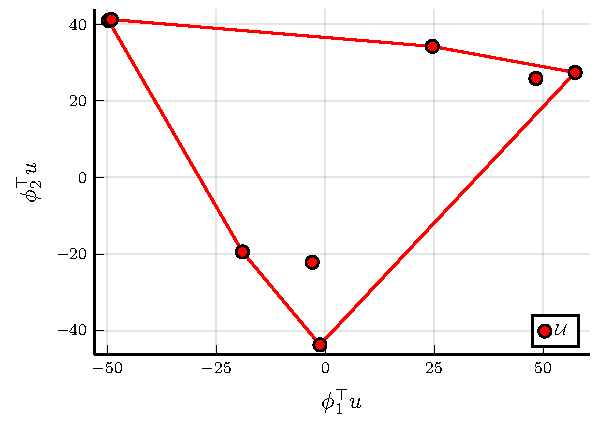
\includegraphics[width=0.45\textwidth]{../notebooks/plots/visual_U.pdf}
    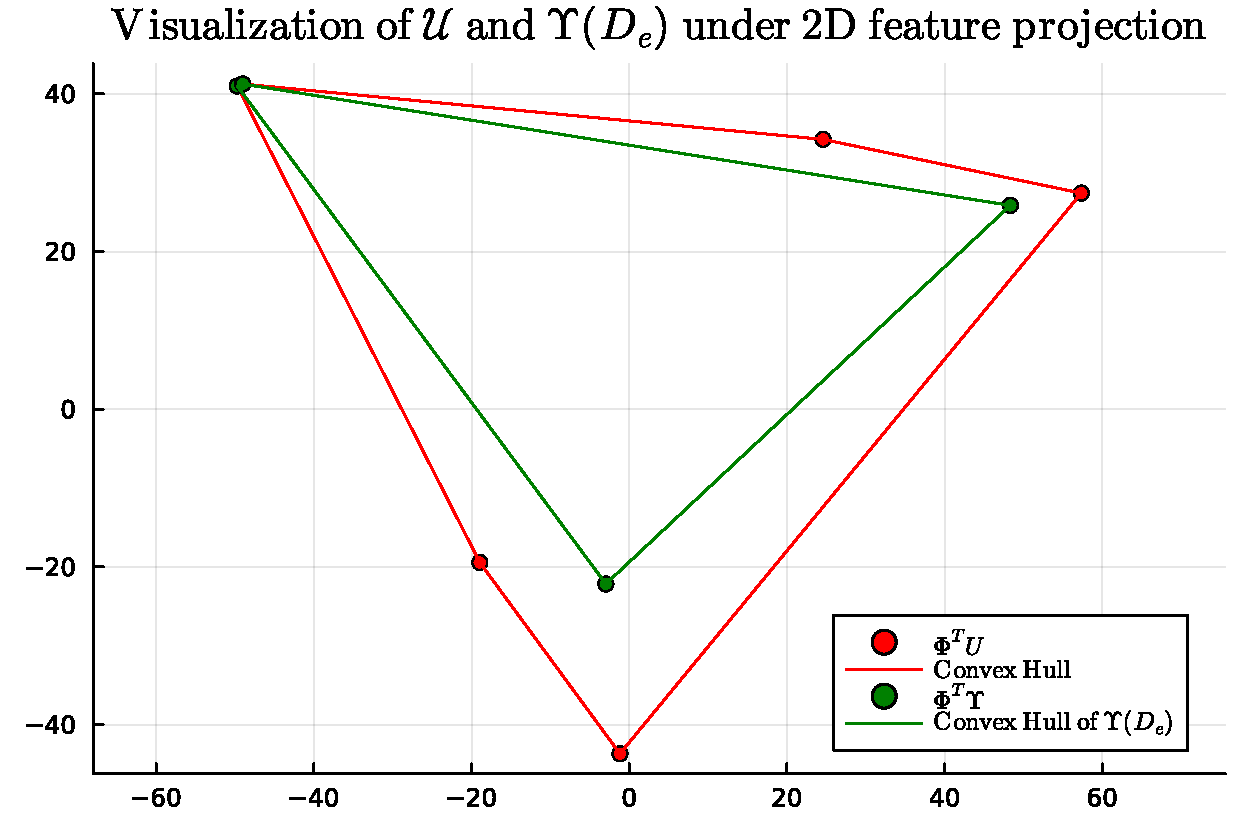
\includegraphics[width=0.45\textwidth]{../notebooks/plots/visual_U_and_Upsilon.pdf}
    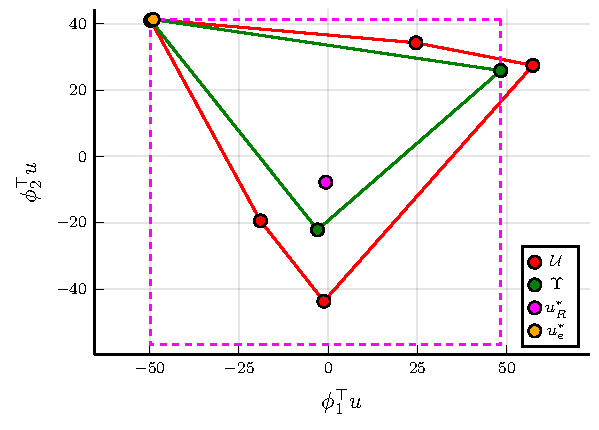
\includegraphics[width=0.45\textwidth]{../notebooks/plots/visual_solve_cheb.pdf}
    %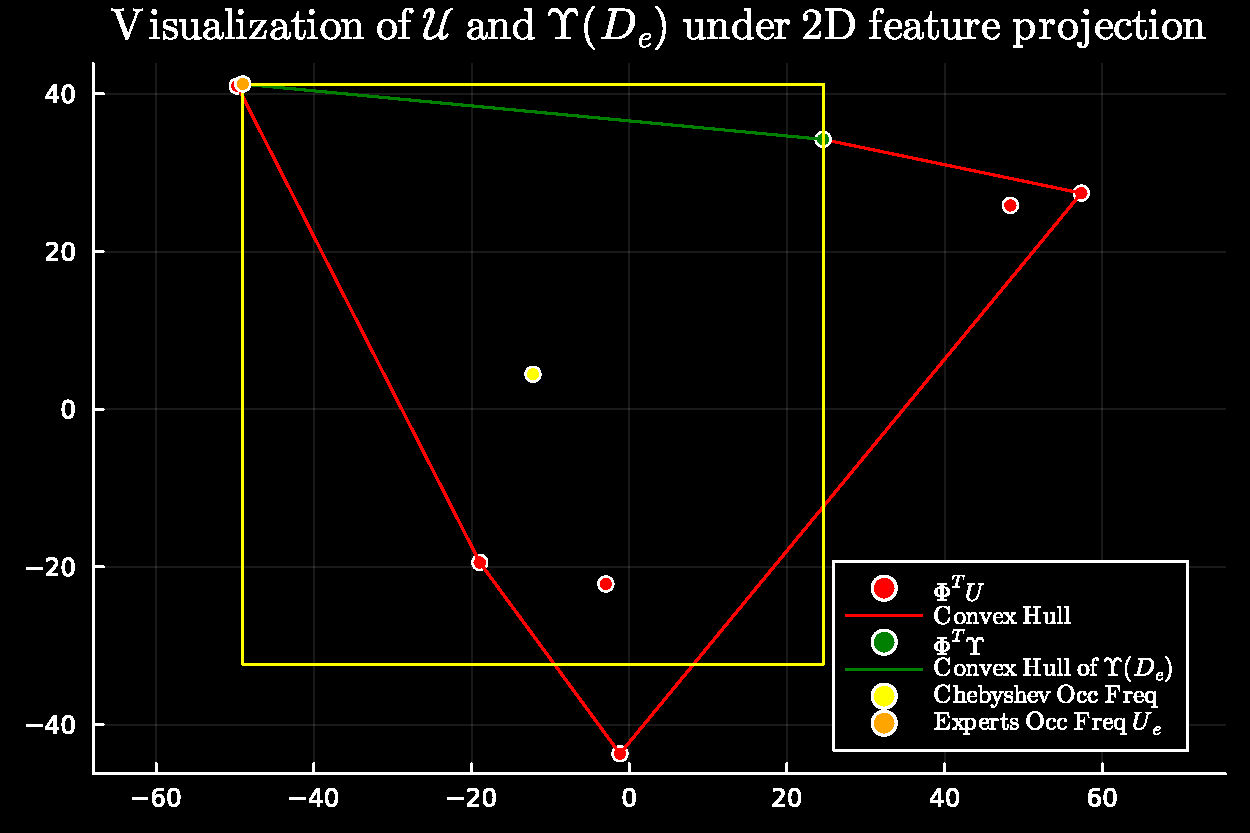
\includegraphics[width=0.45\textwidth]{../notebooks/plots/visual_solve_cheb_outside_upsilon.pdf}
    \caption{Visual depiction of ROIL as a Chebyshev center of the set $\Upsilon$.}
    \label{fig:visual_representation_of_ROIL}
\end{figure}

\section{Covariate Shift Bounds}
\label{sec:covar-shift-bounds}
In this section, we describe an extension of ROIL that allows one to control for the size of the approximation errors in the occupancy frequencies for both states and actions. We begin by expanding our definition of $\Upsilon$ to allow for more general sets.
%
\begin{equation}
    \Upsilon = \{u \in \mathcal{U} \mid g_j(u) \leq 0\}
\end{equation}
%
For example, one might want to model LPAL this way.
%
\begin{equation}
\label{linf_constraint}
	\Upsilon(\mathcal{D}) = \left\{ u \in \mathcal{U} \mid  
 \| (u - \hat{u_e})\tr \Phi \| \le \eps 
 \right\}~.
\end{equation}
\begin{equation}
	\Upsilon(\mathcal{D}) = \left\{ u \in \mathcal{U} \mid  
 \| d_u - \hat{d} \| \le \epsilon_1, 
 \| \pi_u - \hat{\pi} \| \le \epsilon_2
 \right\}~.
\end{equation}
%
Let's try and generalize the above formulation, and lets hold off on applying the dual norm so quickly.
%
\begin{equation}
\begin{aligned}
    \label{eq:new_robust_IRL}
    &\min_{u \in \mathcal{U}} \max_{v \in \Upsilon} \max_{r \in \mathcal{R}} v\tr r - u\tr r \\
    &=\min_{u \in \mathcal{U}} \max_{r \in \ext(\mathcal{R})} \max_{v \in \Upsilon} v\tr r - u\tr r \\
    &=\min_{u \in \mathcal{U}} \max_{r \in \ext(\mathcal{R})} (-u\tr r + \max_{v \in \Upsilon} v\tr r) \\
\end{aligned}
\end{equation}
\begin{equation}
    \begin{mprog}
        \minimize{t \in \Real, u \in \Real^{SA}} t
        \stc t \geq -u\tr r_i + \max_{v \in \Upsilon} v\tr r_i \;\; \forall r_i \in \ext(\mathcal{R})
        \cs A\tr u = p_0
        \cs u \geq 0
    \end{mprog}
\end{equation}

To solve the inner maximization we assume that the constraints on $\Upsilon$ are linear or can be coerced into linear constraints.

\begin{equation}
    \begin{mprog}
        \maximize{v \in \Real^{SA}} v\tr r_i
        \stc A\tr v = p_0
        \cs v \geq 0
        \cs g_j(v) \leq 0
    \end{mprog}
\end{equation}

Let $u_R(\eps)$ be the minimizer of \ref{eq:new_robust_IRL} when the set $\Upsilon$ is defined as in \ref{linf_constraint}, and let $f_R(\eps)$ be the objective value achieved by $u_R(\eps)$.
Let $f_t$ be the objective value of 
%
\[\max_{r\in\mathcal{R}} r\tr (u_e - u_r(\eps))\]
%
then 
%
\[f_t \leq f_R(e_t)\]
\[f_R(\eps_t) = \min_{u \in \Upsilon(\eps_t)} \max_{v \in \Upsilon(\eps_t)} \lvert\lvert \Phi\tr (v-u) \rvert\rvert_\infty\]
\[\geq \min_{\mu \in \mathcal{U}} \lvert\lvert \Phi\tr (u_e - \mu) \rvert\rvert_\infty \geq f_t\]
%  
\begin{restatable}[Regret Bounds]{thm}{roilRegretBound}
\label{roilRegretBound}
The regret of a occupancy frequency $u_R(\eps)$ which minimizes \ref{eq:new_robust_IRL} $\leq \eps_t + \eps$
where $\eps_t = \lvert\lvert \Phi\tr (\hat{u_e} - u_e) \rvert\rvert_\infty$.
\end{restatable}
\begin{proof}
    \[f_t = \max_{r\in\mathcal{R}} r\tr(u_e - u_R(\eps)) = \lvert\lvert \Phi\tr (u_e - u_R(\eps)) \rvert\rvert_\infty \leq \lvert\lvert \Phi\tr (u_e - \hat{u_e} + \hat{u_e} - u_R(\eps)\rvert\rvert_\infty\]
    \[\leq \lvert\lvert \Phi\tr (u_e-\hat{u_e}) \rvert\rvert_\infty + \lvert\lvert \Phi\tr (\hat{u_e} - u_R(\eps)) \rvert\rvert_\infty\]
    \[\leq \eps_t + \eps\]
\end{proof}

\section{Analysis}
\mm{Things to show:
	\begin{enumerate}
		\item When each state is present in the dataset, then we can compute a policy that has zero worst-case regret
		\item What if there is one state that we have not seen, can we bound the regret then?
	\end{enumerate}
 }

Define $\mathcal{D}_S$ to be the set of all states that have been observed in the expert's trajectories:
\[
	\mathcal{D}_S  = \left\{ s\in \mathcal{S} \; \mid \; \exists\; a\in \mathcal{A}, \; (s,a) \in \mathcal{D} \right\}.
\]
%
\begin{restatable}[Expert Recovery]{prop}{expertRecovery}
    \label{expert_recovery}
    If $\mathcal{D}_\mathcal{S} = \mathcal{S}$ then $|\Upsilon(\mathcal{D})| = 1$
    and $u \in \Upsilon(\mathcal{D}) \Rightarrow u = u^{\pi_e}$.
\end{restatable}
%
\begin{proof}
	Given $\mathcal{D}_\mathcal{S} = \mathcal{S}$ then $|\Pi_R(\mathcal{D})| = 1$
	because there can only be one policy consistent with the demonstration
	$\mathcal{D}$ since every state was mapped to an action by $\pi_e \in \Pi_D$
	which generated $\mathcal{D}$. Therefore, by Lemma 1, $u^\pi$ for $\pi \in
		\Pi_R(\mathcal{D})$ is the only occupancy frequency consistent with the
	demonstration, and thus $|\Upsilon(\mathcal{D})| = 1$. By the above
	statements, $u \in \Upsilon(\mathcal{D}) \Rightarrow u = u^{\pi_e}$.
\end{proof}

\paragraph{Limitations of ROIL}
Consider the following deterministic MDP, where $S = \{s_1, s_2, s_3\}$, $A = \{a_1, a_2\}$, $p_0 = [1,0,0]$,
and $\Phi = r^* = [0,0,1,1,-1,-1]$:
\begin{center}
	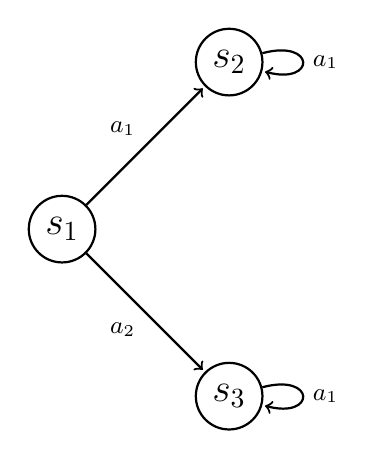
\begin{tikzpicture}[->,shorten >=1pt,auto,node distance=3cm,
			thick,main node/.style={circle,draw,font=\sffamily\Large\bfseries}]

		\node[main node] (1) {$s_1$};
		\node[main node] (2) [above right of=1] {$s_2$};
		\node[main node] (3) [below right of=1] {$s_3$};

		\path[every node/.style={font=\sffamily\small}]
		(1) edge node [above left] {$a_1$} (2)
		edge node [below left] {$a_2$} (3)
		(2) edge [loop right] node {$a_1$} (2)
		(3) edge [loop right] node {$a_1$} (3);
	\end{tikzpicture}
\end{center}

Solving this MDP yields $u_e = [1,0,\frac{\gamma}{1-\gamma},0,0,0]$, however, ROIL fails to find this solution for some datasets.
While other less involved methods like LPAL~\cite{Syed2008} successfully recover $u_e$ no matter the dataset. Take for example
$D = [(s_2, a_1)]$, this causes ROIL to find $u = [\frac{1}{2},\frac{1}{2},\frac{\gamma}{2(1-\gamma)},0,\frac{\gamma}{2(1-\gamma)},0]$.
This example exposes two downsides of ROIL. Firstly, the pessimistic nature of ROIL, it assumes that the expert is trying to maximize the worst-case reward,
and thus its solution randomizes among the actions in the first state. Secondly, ROIL cannot take advantage the number of times that a state action pair is visited,
and therefore what makes a dataset good for LPAL and other occupancy matching methods is not necessarily good for ROIL.

\paragraph{The Strengths of ROIL}

Proposition~\ref{expert_recovery} illustrates the main purpose of our work. The following domain shows what is possibly the greatest strength of our method.
Consider the following deterministic MDP, where $S = \{s_1, s_2\}$, $A_{s_1} = \{a_1, a_2\}$, $A_{s_2} = \{a_1\}$, $p_0 = [1-\epsilon,\epsilon]$,
and the choice of $\Phi$ is of no consequence:
\begin{center}
	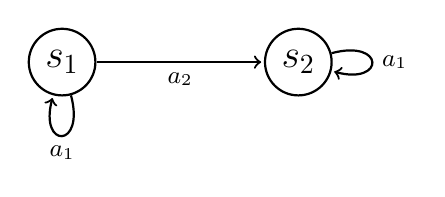
\begin{tikzpicture}[->,shorten >=1pt,auto,node distance=3cm,
			thick,main node/.style={circle,draw,font=\sffamily\Large\bfseries}]

		\node[main node] (1) {$s_1$};
		\node[main node] (2) [right of=1] {$s_2$};

		\path[every node/.style={font=\sffamily\small}]
		(1) edge [loop below] node {$a_1$} (1)
		(1) edge node [below, midway] {$a_2$} (2)
		(2) edge [loop right] node {$a_1$} (2);
	\end{tikzpicture}
\end{center}

Consider an optimal occupancy frequency $u^*_e = [\frac{\epsilon + \gamma - 1}{\epsilon(1-\gamma)}, 0, \frac{1}{\epsilon}]$ which generates a dataset $D = [(s1, a1), (s2, a1)]$
this leads both LPAL and GAIL to estimate $\hat{u}_e = [\frac{1}{2(1-\gamma)}, 0, \frac{1}{2(1-\gamma)}]$. One can verify that the set of occupancy frequencies
for this domain can be represented as a convex combination of the two deterministic policies resulting in
\[U = \{\xi[\frac{\epsilon+\gamma-1}{\epsilon(1-\gamma)}, 0, \frac{1}{\epsilon}] + (1-\xi)[0,1-\epsilon,\frac{\gamma}{1-\gamma}+\epsilon] \;\mid\; \xi \in [0,1]\}\] 
Now we show that minimizing either the GAIL or LPAL objective given the above dataset does not converge to $u^*_e$. While by Proposition~\ref{expert_recovery} ROIL is guaranteed to recover the expert.

\begin{figure}[htbp]
	\centering
	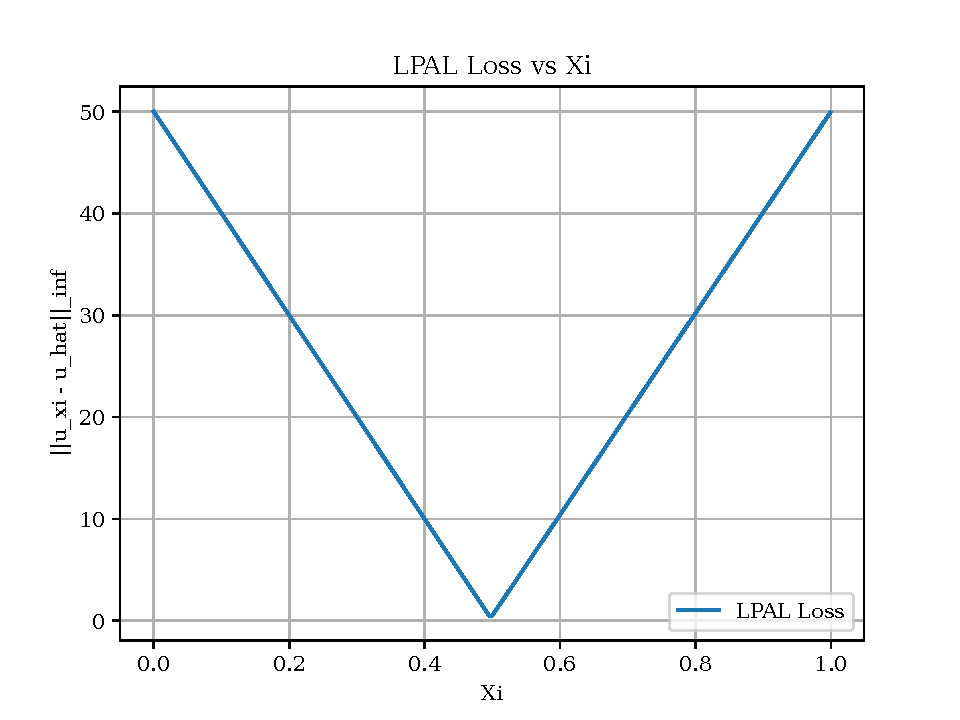
\includegraphics[width=0.45\textwidth]{../src/plots/all_state/lpal_loss.pdf}
	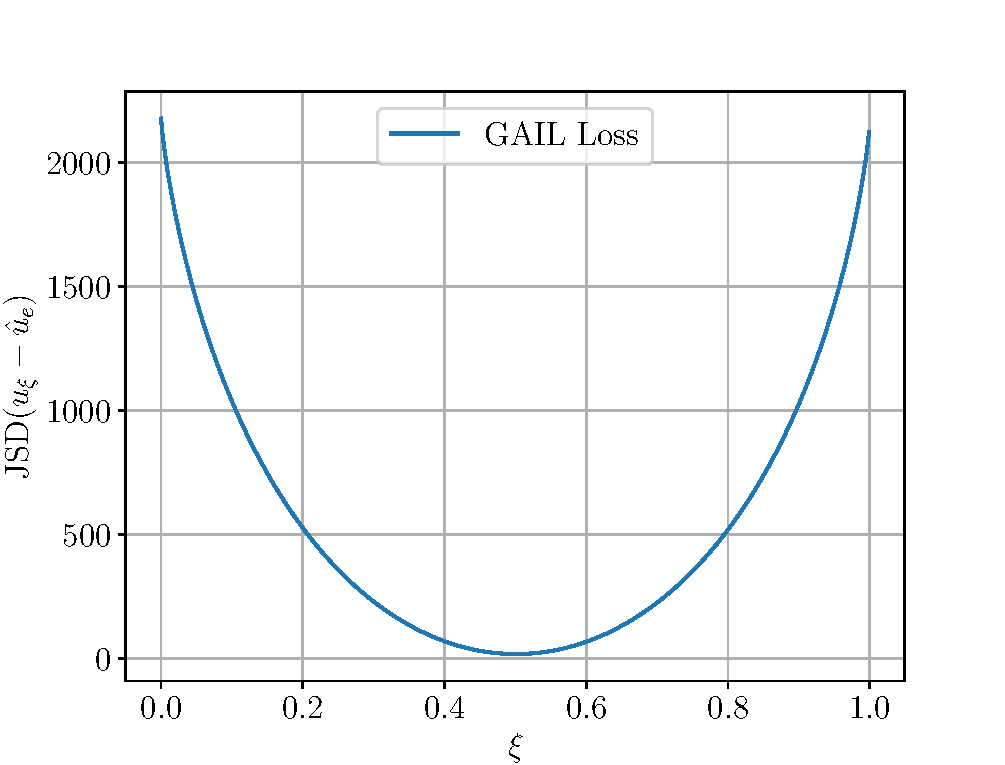
\includegraphics[width=0.45\textwidth]{../src/plots/all_state/gail_loss.pdf}
	\caption{The loss functions of LPAL and GAIL. Here JSD refers to the Jensen-Shannon Divergence which is the loss function minimized by GAIL when the coefficient of the 
 causal entropy term H is 0~\cite{Ho2016}.}
	\label{fig:loss_of_LPAL_GAIL}
\end{figure}


\section{Experimental Results}
\label{sec:experimental-results}
\begin{enumerate}
	\item Discuss our experiments using the above defined algorithms.
	\item Discuss whether our algorithm meets its analytical results.
	\item Demonstrate its performance on up-to-date sandboxes.
\end{enumerate}

\begin{figure}[htbp]
	\centering
	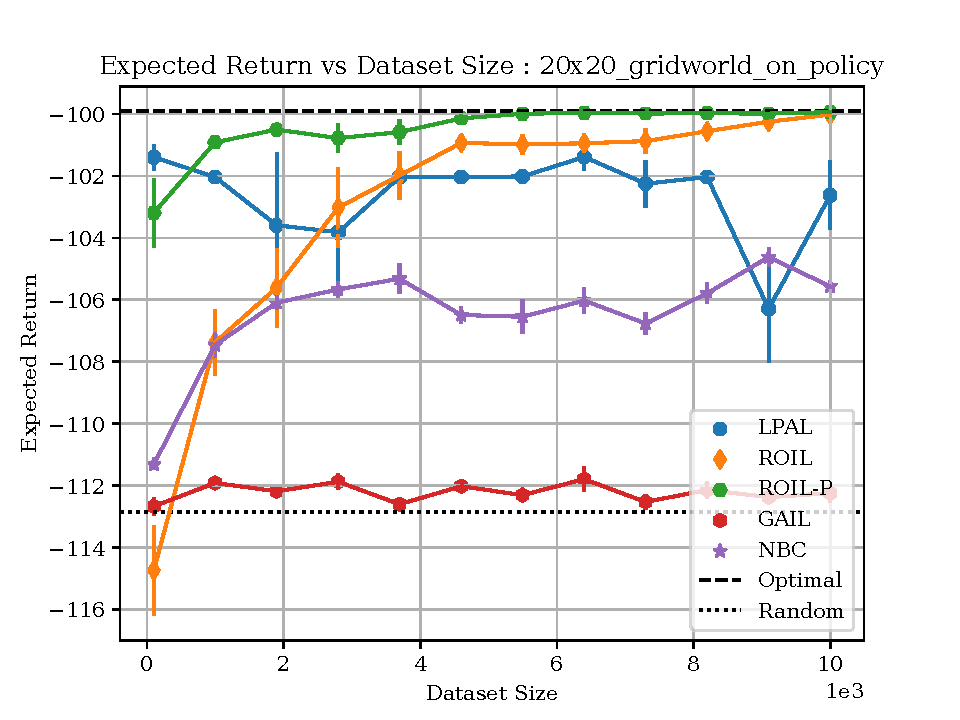
\includegraphics[width=0.45\textwidth]{../src/plots/returns/20x20_gridworld_on_policy_returns.pdf}
	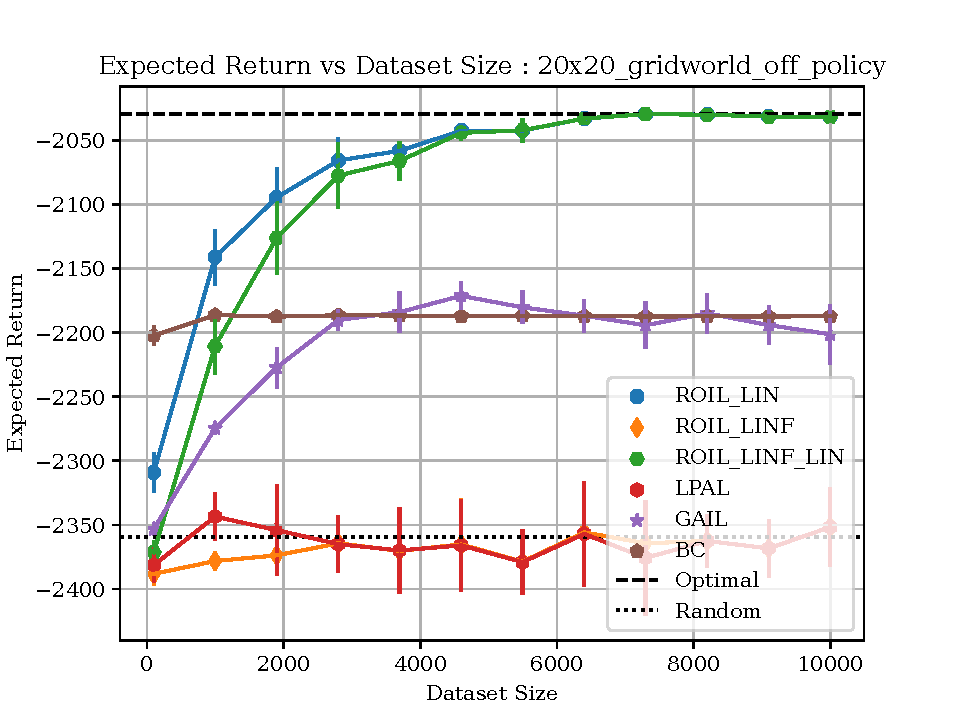
\includegraphics[width=0.45\textwidth]{../src/plots/returns/20x20_gridworld_off_policy_returns.pdf}
	\caption{On and off policy performance of IRL methods on 20x20 grid world}
	\label{fig:off_policy_vs_on_20}
\end{figure}

\begin{figure}[htbp]
	\centering
	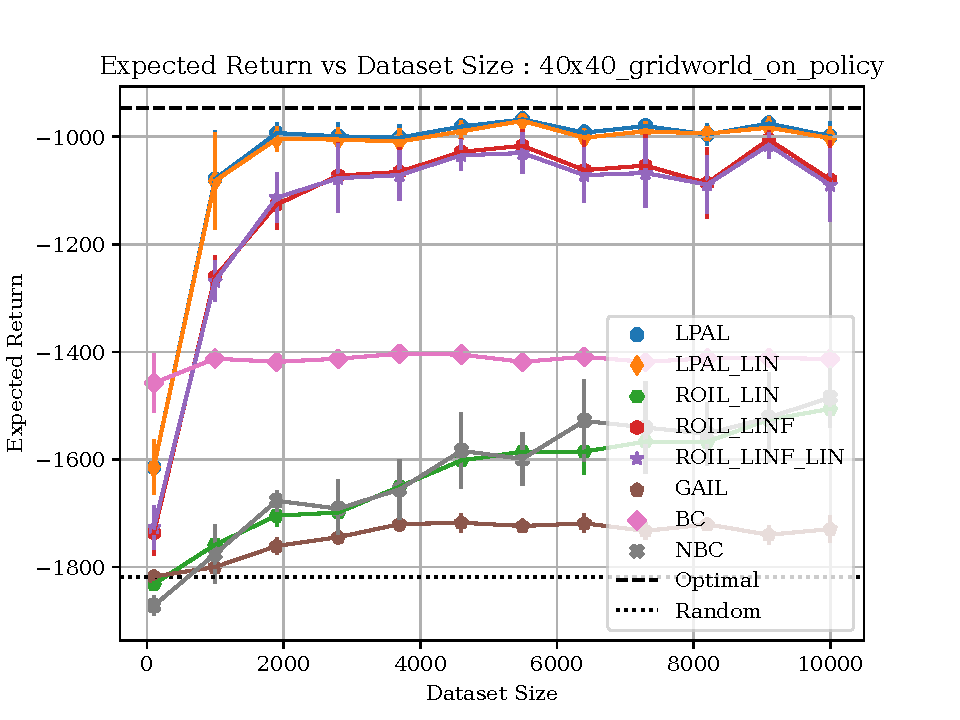
\includegraphics[width=0.45\textwidth]{../src/plots/returns/40x40_gridworld_on_policy_returns.pdf}
	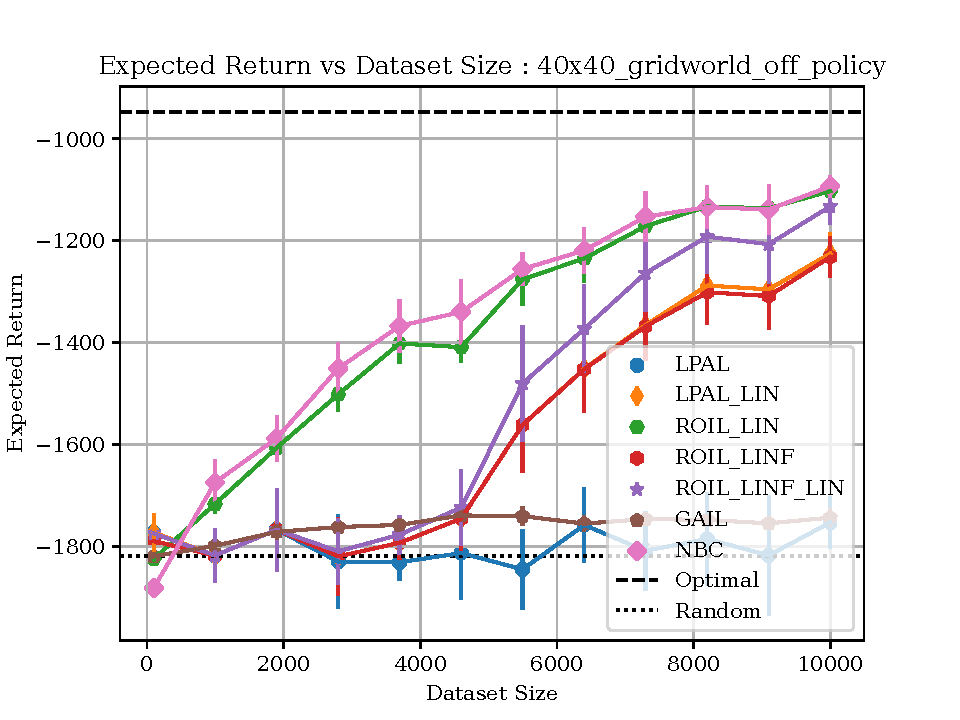
\includegraphics[width=0.45\textwidth]{../src/plots/returns/40x40_gridworld_off_policy_returns.pdf}
	\caption{On and off policy performance of IRL methods on 40x40 grid world}
	\label{fig:off_policy_vs_on_40}
\end{figure}

\section{Conclusion}
% \begin{enumerate}
% 	\item Restate the main idea that lead us to this problems' solution.
% 	\item Restate the performance of our method.
% 	\item Outline where these ideas could be applied in the future.
% \end{enumerate}
Our insight into the IL problem has been that it is not necessary to approximate the expert through the application of the Chebyshev approximation to solve the robust IL formulation. 
Our method performs well even when the demonstrations come from a different state visitation policy.
The LP we proposed can be large, however efficiently solved as many other LPs are.
In future works, we hope to study other methods for robustness in IL as well as other areas of research that could benefit from our insights.

%\bibliographystyle{plain}
\bibliography{irl.bib}

\section{Appendix}
\lemmaOccupancyExistance*
\begin{proof}
	To do this, we use the policy to occupancy frequency correspondence~\cite{Puterman1994}.
	\[\forall \pi \in \Pi \,\,\,\, u^\pi(s,a) = \pi(a|s)\sum_{a'}{u^\pi(s,a')}\]

	Case 1: Prove $u \in \Upsilon (\mathcal{D})  \quad \Rightarrow \quad  \exists
		\pi \in \Pi_R(\mathcal{D}), \, u = u^{\pi}$,

	Given $u \in \Upsilon (\mathcal{D})\,\,$ constructing policy $\pi$ from
	occupancy frequency $u$ via the policy occupancy correspondence we have.

	\[\pi(a|s) = \frac{u(s,a)}{\sum_{a`}u(s,a`)}\]

	Since $u \in \Upsilon (\mathcal{D})$, $u\tr c = 0$ for some $c \in \Real^{SA}$ such that
	$c(s,a) = 1$ if $(s,\cdot) \in \mathcal{D}, (s,a) \notin \mathcal{D}$ and $c(s,a) = 0$ otherwise.
	Therefore, for states $s$ where $(s,\cdot) \in \mathcal{D}$ we have $u(s,a) = 0$ for all $a \not= \pi_e(s)$.
	Only one action for that state will be non-zero, therefore for observed states we have $\pi(a|s) = 1$.

	Case 2: Prove $\pi \in \Pi_R(\mathcal{D}) \quad \Rightarrow \quad  u^\pi \in
		\Upsilon (\mathcal{D})$

	Given that $\pi \in \Pi_R(\mathcal{D})$, $\pi(a|s) = 1$ for all $(s,a) \in \mathcal{D}$. Therefore, for observed states $s$, $u(s,a) = 0$ for all $a \not= \pi_e(s)$
	since $u(s,a) = \pi(a|s)\sum_{a'}{u^\pi(s,a')}$. Then we see that indeed for the $c$ as defined in case 1, $u\tr c = 0$.
\end{proof}

\chebeyshevRegret*
\begin{proof}
	For the sake of contradiction,
	assume there exists some $\pi' \in \Pi$ such that
	\[
		\max_{r\in \mathcal{R}} \max_{\pi \in \Pi_{R}(\mathcal{D})}
		\left(\rho(\pi,r) - \rho(\pi', r)\right) < \max_{r\in \mathcal{R}}
		\max_{\pi \in \Pi_{R}(\mathcal{D})}
		\left(\rho(\pi, r) - \rho(\hat{\pi}, r)\right)
	\]
	After algebraic manipulation, we have
	\begin{align*}
		\max_{r\in \mathcal{R}} \max_{\pi \in \Pi_{R}
			(\mathcal{D})} u_{\pi}\tr r - u_{\pi'}\tr r
		 & < \max_{r\in \mathcal{R}}
		\max_{\pi \in \Pi_{R}
			(\mathcal{D})} u_{\pi}\tr r - u_{\hat{\pi}}
		\tr r                                              \\
		\max_{r\in \mathcal{R}} \max_{\pi \in \Pi_{R}(\mathcal{D})}
		(u_{\pi} - u_{\pi'})\tr r
		 & < \max_{r\in \mathcal{R}}
		\max_{\pi \in \Pi_{R}(\mathcal{D})}
		(u_{\pi} - u_{\hat{\pi}})\tr r
		\\
		\max_{w\in \mathcal{W}} \max_{v \in \Upsilon} (v - u_{\pi'})\tr \Phi w
		 & < \max_{w\in \mathcal{W}} \max_{v \in \Upsilon}
		(v - u_{\hat{\pi}})\tr \Phi w
	\end{align*}
	Here, $u_{\pi}$, $u_{\pi'}$, and $u_{\hat{\pi}}$
	are the occupancy frequencies of their respective policies.

	Notice the change in the maximization objectives.
	We assume that $r = \Phi\tr w$ for some $w \in \mathcal{W}$,
	thus the maximization over $\mathcal{R}$ is equivalent to the maximization
	over $\mathcal{W}$ of $\Phi\tr w$.
	Secondly, by the occupancy frequency correspondence~\cite{Puterman1994}, the
	maximization over $\Pi_R(\mathcal{D})$ is equivalent to the maximization over
	$\Upsilon$.
	Since $u_{\hat{\pi}} \in \arg\min_{u \in \mathcal{U}} \max_{w \in \mathcal{W}} \max_{v \in \Upsilon} {(v - u)}^T \Phi w$,
	this is a contradiction with the optimality of $\hat{\pi}$,
	therefore $\pi'$ cannot achieve less regret than $\hat{\pi}$.
\end{proof}

\roilLp*
\begin{proof}
    Recall the definition of $\Phi \in \Real^{SA \times K}$ given some arbitrary ordering on $(s,a)$ pairs.
    \begin{center}
    
    	\[\*\Phi\tr \;=\; \begin{bmatrix}
    			- & \phi_1\tr & - \\
    			- & \phi_2\tr & - \\
    			- & \vdots    & - \\
    			- & \phi_K\tr & -
    		\end{bmatrix}\]
    
    	Where $\phi_n = [\phi_n(s,a)\;\;\forall s,a \in S \times A]$ represents the n'th feature evaluated on each $(s,a)$ pair.
    \end{center}
    
    We apply a technique called Chebyshev Approximation~\cite{boyd_convex_optimization}(6.1) to equation~\eqref{eq:extreme_points_of_the_IRL_Formulation}.
    This step can also be seen as writing~\eqref{eq:extreme_points_of_the_IRL_Formulation} in epigraph form.
    
    \begin{equation}
    	\begin{mprog}
    		\minimize{u \in \mathcal{U}, \sigma \in \Real} \sigma
    		\stc \max_{v \in \Upsilon} |(v - u)\tr \Phi_i| \leq \sigma
    		\cs i \in 1 \dots k
    	\end{mprog}
    \end{equation}
    
    After expanding the absolute value is equivalent to.
    
    \begin{equation}
    	\begin{mprog}
    		\minimize{u \in \mathcal{U}, \sigma \in \Real} \sigma
    		\stc \max_{v \in \Upsilon} (v - u)\tr \Phi_i \leq \sigma
    		\cs \max_{v \in \Upsilon} -(v - u)\tr \Phi_i \leq \sigma
    		\cs i \in 1 \dots k
    	\end{mprog}
    \end{equation}
    
    In order to make the above problem more easily solvable, let us take the dual of the first inner maximization problem.
    
    \begin{equation}
    	\begin{mprog}
    		\maximize{v \in \Upsilon} (v - u)\tr \Phi_i
    		\cs i \in 1\dots k
    	\end{mprog}
    \end{equation}
    
    Notice in order to get this into an LP form we need to take the convex set $\Upsilon$ and construct a linear constraint which encapsulates what it means for an element $v \in \Real_+^{SA}$ to be in the set $\Upsilon$. Luckily this is easy to do as $\Upsilon$ is defined as a linear constraint on $\mathcal{U}$. For the sake of simplicity suppose that we consider one fixed $\Phi_i$, and omit the optimization over all $i \in 1\dots k$ for the duration
    of the dual derivation. But do keep in mind, each feature vector gets its own dual variable.
    
    \begin{equation}
    	\label{eq:primal_IRL_problem}
    	\begin{mprog}
    		\maximize{v \in \Real_+^{SA}} (v - u)\tr \Phi_i
    		\stc c\tr v = 0
    		\cs \sum_{a \in \mathcal{A}}(I - \gamma P_a\tr)v(\cdot, a) = p_0
    	\end{mprog}
    \end{equation}
    
    \begin{equation}
    	L(v, \alpha, \beta) = (v - u)\tr \Phi_i + \alpha c\tr v
    	+ \beta\tr (\sum_{a \in \mathcal{A}}(I - \gamma P_a\tr)v(\cdot, a) - p_0)
    \end{equation}
    
    Writing the summation as a matrix-vector multiplication we have.
    
    \[\*A \;=\; \begin{bmatrix}
    		- & (I - \gamma P_1) & - \\
    		- & (I - \gamma P_2) & - \\
    		- & \vdots           & - \\
    		- & (I - \gamma P_a) & - \\
    	\end{bmatrix}\;\in\; \Real^{SA\times S}\]
    
    \begin{equation}
    	\label{eq:rewrite_U_constraint}
    	L(v, \alpha, \beta) = (v - u)\tr \Phi_i + \alpha c\tr v
    	+ \beta\tr (A\tr v - p_0)
    \end{equation}
    
    Notice that we assume that the vector $v \in \Real^{SA}$ iterates over states first before iterating over actions.
    
    \begin{equation}
    	g(\alpha, \beta) = \sup_{v\geq 0} L(v, \alpha, \beta)
    \end{equation}
    
    \begin{equation}
    	g(\alpha, \beta) = -u\tr \Phi_i - \beta\tr p_0 + \sup_{v\geq 0} (v\tr \Phi_i + \alpha c\tr v + \beta\tr A\tr v)
    \end{equation}
    
    \begin{equation}
    	g(\alpha, \beta) = -u\tr \Phi_i - \beta\tr p_0 + \sup_{v \geq 0} (\Phi_i\tr + \alpha c\tr + \beta\tr A\tr)v
    \end{equation}
    
    Notice that the quantity in the parentheses is linear in $v$, and linear functions are
    bounded above if and only if their coefficient is 0.
    Therefore, $g(\alpha, \beta) = \infty$ except for when $\Phi_i + \alpha c + A\beta \leq 0$ in which case
    $g(\alpha, \beta) = -u\tr \Phi_i - \beta\tr p_0$.
    
    Now we are ready to define the dual of~\eqref{eq:primal_IRL_problem}.
    Given that $g(\alpha, \beta)$ is an upper bound on the optimal value of~\eqref{eq:primal_IRL_problem} for feasible $v$, we wish to minimize it.
    
    \begin{equation}
    	\begin{mprog}
    		\minimize{\alpha \in \Real, \beta \in \Real^{S}} -u\tr \Phi_i - \beta\tr p_0
    		\stc \Phi_i + \alpha c + A\beta \leq 0
    	\end{mprog}
    \end{equation}
    
    Recall the formulation of the Chebyshev Center.
    \begin{equation}
    	\begin{mprog}
    		\minimize{u \in \mathcal{U}, \sigma \in \Real} \sigma
    		\stc \max_{v \in \Upsilon} (v - u)\tr \Phi_i \leq \sigma
    		\cs \max_{v \in \Upsilon} -(v - u)\tr \Phi_i \leq \sigma
    		\cs i \in 1 \dots k
    	\end{mprog}
    \end{equation}
    
    Now derive a similar result for the second maximization using the same method as above and substitute.
    Recall that each feature-vector has its own unique dual variables.
    
    \begin{equation}
    	\begin{mprog}
    		\minimize{u\in\mathcal{U}, \sigma\in\Real} \sigma
    		\stc \min_{\alpha_i \in \Real, \beta_i \in \Real^{S}} -u\tr \Phi_i - \beta_i\tr p_0 \leq \sigma
    		\cs \Phi_i + \alpha_i c + A \beta_i \leq 0
    		\cs \min_{\hat{\alpha}_i \in \Real, \hat{\beta}_i \in \Real^{S}} u\tr \Phi_i - \hat{\beta}_i\tr p_0 \leq \sigma
    		\cs -\Phi_i + \hat{\alpha}_i c + A \hat{\beta}_i \leq 0
    		\cs i \in 1 \dots k
    	\end{mprog}
    \end{equation}
    
    \begin{equation}
    	\begin{mprog}
    		\label{eq:semi_fininished_LP}
    		\minimize{u\in\mathcal{U}, \sigma, \alpha_i, \hat{\alpha}_i \in \Real, \beta_i, \hat{\beta}_i \in \Real^{S}} \sigma
    		\stc -u\tr \Phi_i - \beta_i\tr p_0 \leq \sigma
    		\cs u\tr \Phi_i - \hat{\beta}_i\tr p_0 \leq \sigma
    		\cs \Phi_i + \alpha_i c + A \beta_i \leq 0
    		\cs -\Phi_i + \hat{\alpha}_i c + A \hat{\beta}_i \leq 0
    		\cs i \in 1 \dots k
    	\end{mprog}
    \end{equation}
    
    And now for the final push, notice that~\eqref{eq:semi_fininished_LP} is not an LP,
    because of the nonlinear (yet convex) minimization over $u\in\mathcal{U}$. To remedy this notice
    how we re-wrote the definition of $\mathcal{U}$ in~\eqref{eq:rewrite_U_constraint}. This leads us to the
    LP formulation of the Chebyshev Center.
    \gersi{TODO go back and explain why the $A^{T}v$ constraint makes sense}
    
    \begin{equation}
    	\begin{mprog}
    		\minimize{\sigma, \alpha_i, \hat{\alpha}_i \in \Real, \beta_i, \hat{\beta}_i \in \Real^{S}, u \in \Real^{SA}} \sigma
    		\stc -u\tr \Phi_i - \beta_i\tr p_0 \leq \sigma
    		\cs u\tr \Phi_i - \hat{\beta}_i\tr p_0 \leq \sigma
    		\cs \Phi_i + \alpha_i c + A \beta_i \leq 0
    		\cs -\Phi_i + \hat{\alpha}_i c + A \hat{\beta}_i \leq 0
    		\cs i \in 1 \dots k
    		\cs A\tr u = p_0
    		\cs u \geq 0
    	\end{mprog}
    \end{equation}
\end{proof}

\paragraph{Relationship With LPAL, Syed and Schapire~\cite{Syed2008}}

Theorem 5 of the LPAL paper~\cite{Syed2008} provides a bound on the performance of the policy returned by LPAL.
In this section, we would like to provide insight into this bound using the notation of this paper.

\begin{restatable}[LPAL bound]{thm}{LPAL}
\label{thm:LPAL}
	Let $\pi_{lp}$ be the policy returned by LPAL then
	\[V(\pi_{lp}) \geq V(\pi_e) + v^* - 2\eps\]
	or equivalently expressed using occupancy frequencies
	\[u_{lp}\tr r \geq u_e\tr r + v^* - 2\eps\]

	Where $\eps = \lvert\lvert \hat{u}_e\tr \Phi - u_e\tr \Phi\rvert\rvert_*$
\end{restatable}
\begin{proof}
	Begin with the definitions
	\[
		u^* = \arg\min_{u \in \mathcal{U}} \lvert\lvert u\tr \Phi - \hat{u_e}\tr \Phi \rvert\rvert_*
	\]
	\[
		v^* = - \lvert\lvert \Phi\tr u^* - \Phi\tr \hat{u_e} \rvert\rvert_*
	\]
	Given that we wish to bound $V(\pi_{lp}) - V(\pi_e)$ lets begin with the definition of $V(\cdot)$.
	\[V(\pi_{lp}) - V(\pi_e) = u_{lp}\tr r - u_e\tr r\]
	Both LPAL and our paper assumes that $r = \Phi\tr w$ for some $w \in \mathcal{W} = \Real_{1}$ LPAL calls the columns of $\Phi$ basis
	reward vectors, while we call them features but they are the same, save for notation.
	\[\geq \min_{w \in \mathcal{W}}(u_{lp}\tr \Phi w - u_e\tr \Phi w) =- \max_{w \in \mathcal{W}}(u_e\tr \Phi - u_{lp}\tr \Phi)w \]
	Applying the definition of the dual norm with respect to $\mathcal{W}$
	\[= -\lvert\lvert u_e\tr \Phi - u_{lp}\tr \Phi \rvert\rvert_*\]
	Now we apply the triangle inequality by adding 0
	\[= -\lvert\lvert u_e\tr \Phi - \hat{u}_e + \hat{u}_e - u_{lp}\tr \Phi \rvert\rvert_*\]
	\[\geq -\lvert\lvert u_e\tr \Phi - \hat{u}_e\rvert\rvert_* - \lvert\lvert \hat{u}_e - u_{lp}\tr \Phi \rvert\rvert_* = -\eps - \lvert\lvert \hat{u}_e - u_{lp}\tr \Phi \rvert\rvert_* \]
	\[\geq -\eps - \lvert\lvert \hat{u}_e\tr \Phi - \Phi\tr u^*\rvert\rvert_*\]
	\[= -\eps - \lvert\lvert \hat{u}_e\tr \Phi - u_e\tr\Phi + u_e\tr\Phi - \Phi\tr u^*\rvert\rvert_*\]
	\[\geq -\eps - \lvert\lvert \hat{u}_e\tr \Phi - u_e\tr\Phi\rvert\rvert_* - \lvert\lvert u_e\tr\Phi - \Phi\tr u^*\rvert\rvert_*\]
	\[= -2\eps - \lvert\lvert u_e\tr\Phi - \Phi\tr u^*\rvert\rvert_* = -2\eps + v^*\]
\end{proof}
\end{document}
%%% Local Variables:
%%% mode: LaTeX
%%% TeX-master: t
%%% End:
